\documentclass{beamer}
\usetheme{Madrid} % My favorite!
\setbeamercovered{invisible}
% To remove the navigation symbols from 
% the bottom of slides%
\setbeamertemplate{navigation symbols}{} 
%
\usepackage{enumerate}
\usepackage{graphicx}
\usepackage{subfig}
\usepackage{caption}
\usepackage{wrapfig}

\captionsetup{figurename=,justification=justified}
\graphicspath{{figures/}}



%\usepackage{bm} % For typesetting bold math (not \mathbold)
%\logo{\includegraphics[height=0.6cm]{yourlogo.eps}}
%
\title[Anchor Placement]{Anchor Node Placement for Localization in Wireless Sensor Networks}
\author{Ben Tatham}
\institute[Carleton University]
{
Carleton University \\
Ottawa-Carleton Institute for
Electrical and Computer Engineering \\
\emph{tatham@ieee.org}
}
\date{January 19, 2011}
% \today will show current date. 
% Alternatively, you can specify a date.
%
\begin{document}
%
\begin{frame}
\titlepage
\end{frame}
%
\begin{frame}{Motivation}
\begin{block}{Why Wireless Sensor Networks?}
\begin{columns}
	\begin{column}[T]{0.5\textwidth}
		\begin{figure}
			\centering
				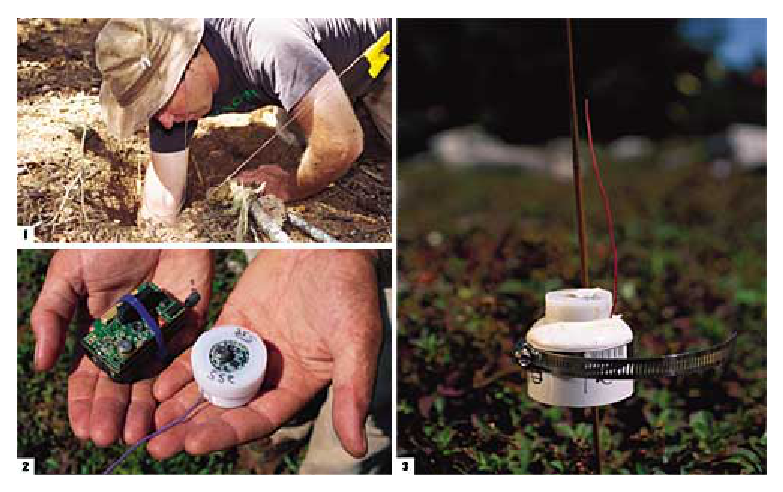
\includegraphics[width=\textwidth]{0404birdf4_123}
				\caption{Great Duck Island\\IEEE Spectrum April 2004}
		\end{figure}
		\vfill
	\end{column}
	\begin{column}[T]{0.5\textwidth}
		\begin{figure}
			\centering
				
\includegraphics[width=0.4\textwidth]{runes_logo}
				\caption{Road tunnel fire rescue\\with the Internet of Things\\YouTube November 2006}
		\end{figure}
		\vfill
	\end{column}
\end{columns}
\end{block}
\end{frame}
%
\begin{frame}{Motivation}
\begin{columns}
	\begin{column}[T]{0.3\textwidth}
		\begin{itemize}
			\item Top row differences are decent
			\item Bottom left: getting worse
			\item Bottom right: what is going on here?
			\item[$\Rightarrow$] What can network designers do?
		\end{itemize}
	\end{column}
	\begin{column}[T]{0.7\textwidth}
		\begin{figure}
		\centering
			\subfloat{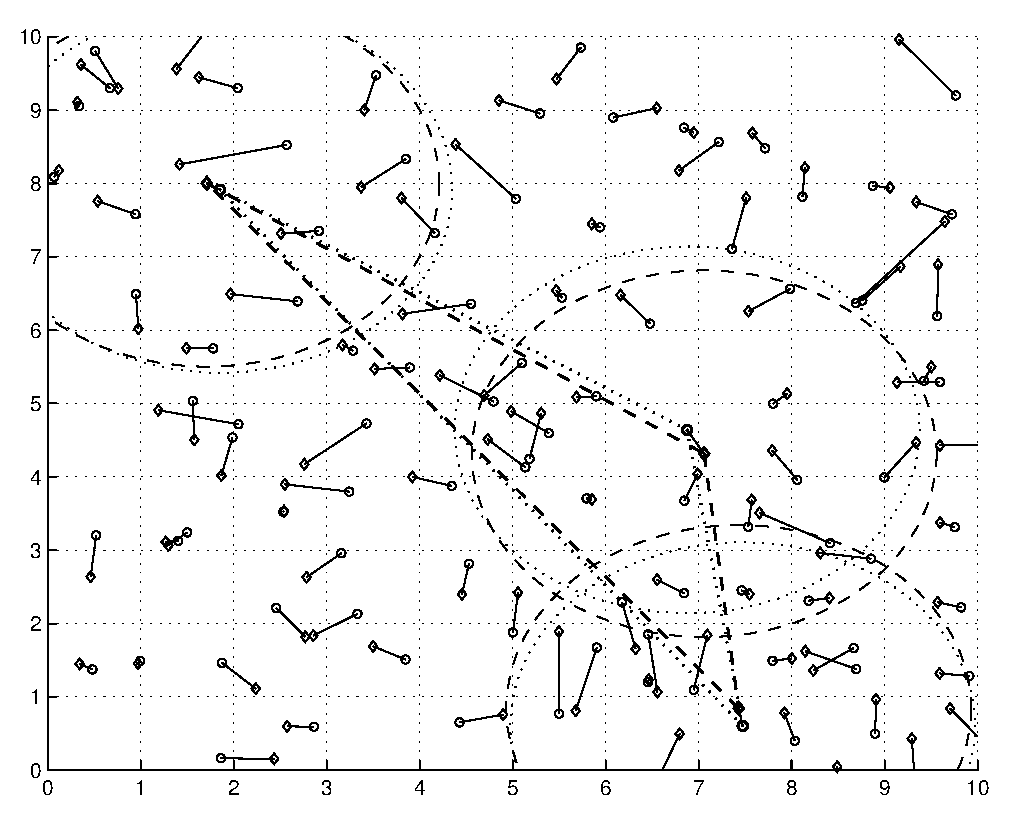
\includegraphics[width=0.45\textwidth]{motivation/plot1}}
			\subfloat{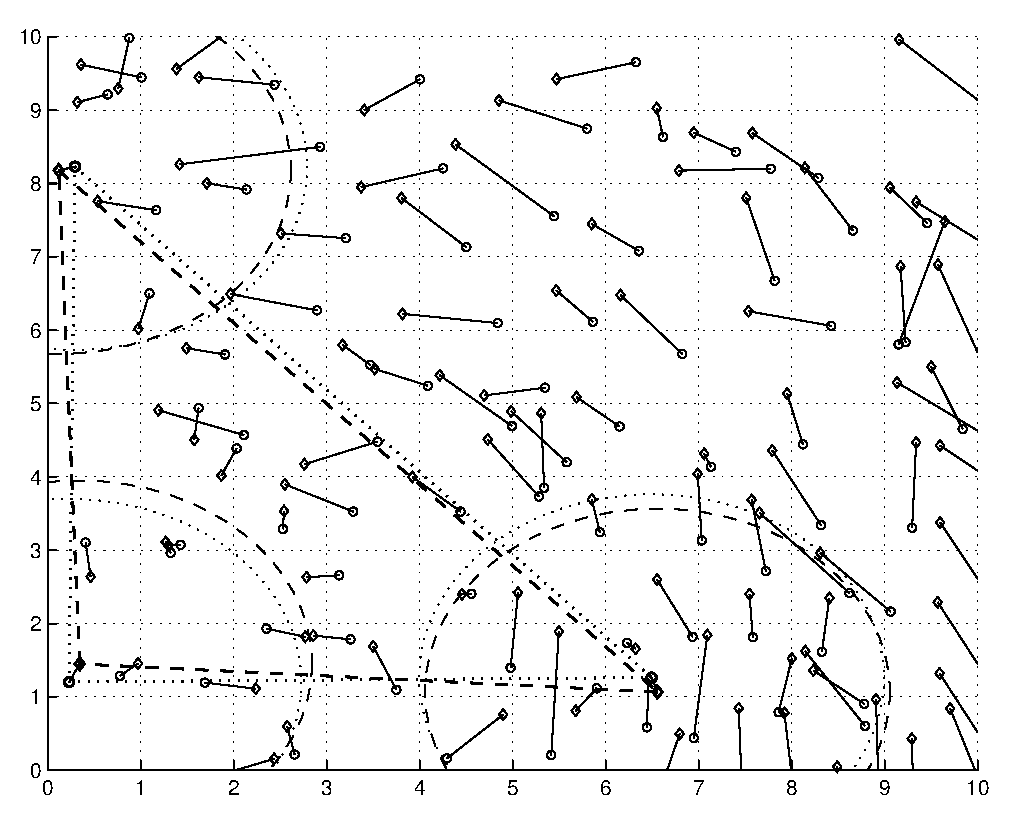
\includegraphics[width=0.45\textwidth]{motivation/plot2}}
			\\
			\subfloat{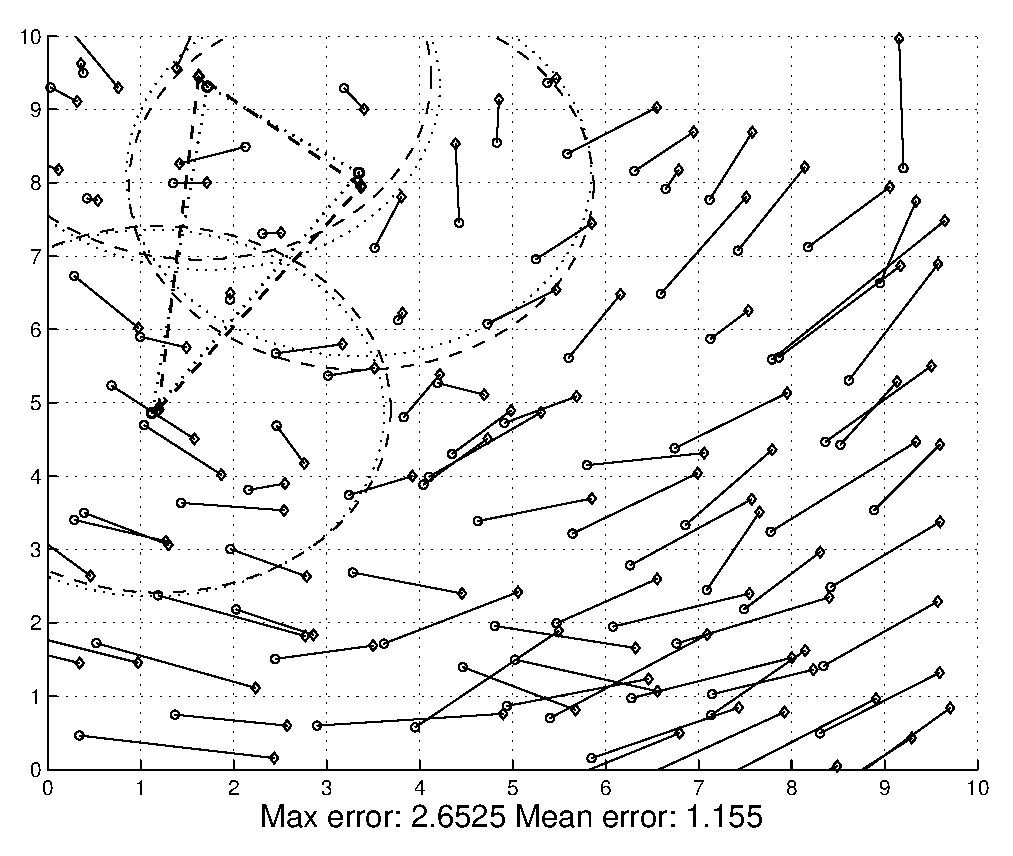
\includegraphics[width=0.45\textwidth]{motivation/plot3}}
			\subfloat{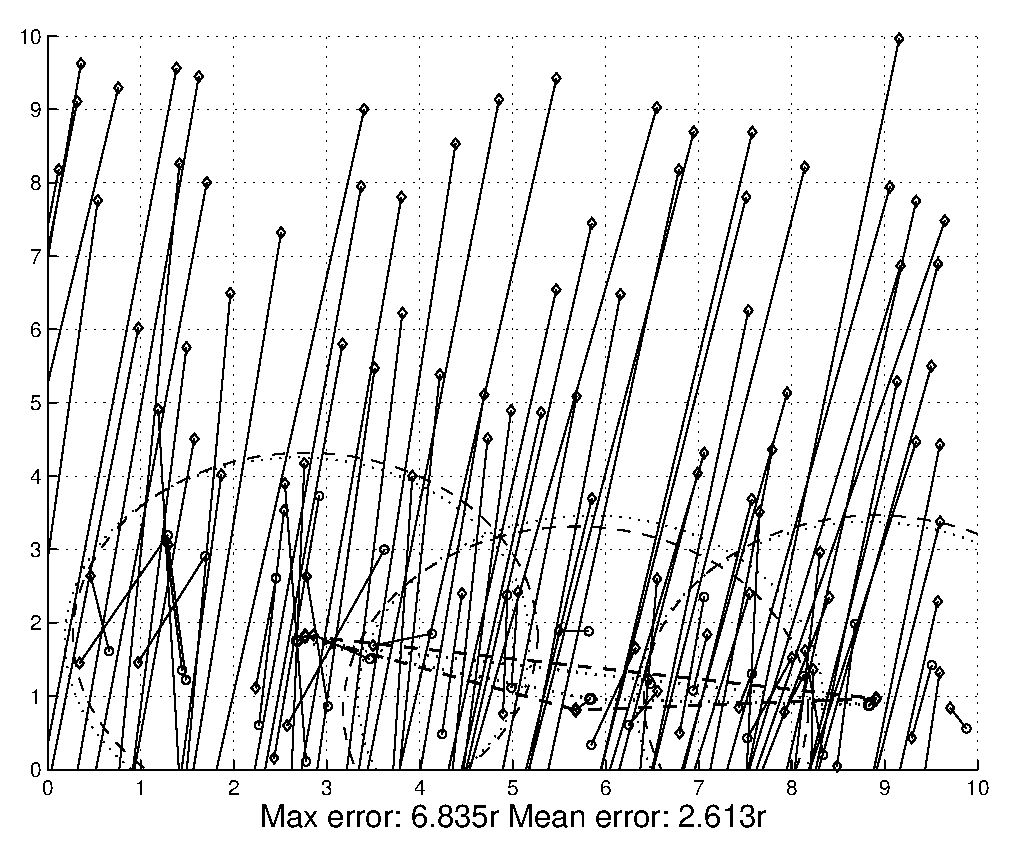
\includegraphics[width=0.45\textwidth]{motivation/plot4}}
		\end{figure}
    \end{column}
\end{columns}
\end{frame}

\begin{frame}{The Basics}
\begin{block}{What are we actually doing?}
\begin{columns}
	\begin{column}[T]{0.3\textwidth}
		\begin{itemize}
		\item Local~$\Rightarrow$ global coordinates
		\item Find best linear transformation
		\item $Z = b \times Y \times T + c$
		\item Procrustes Analysis
			\begin{itemize}
				\item Built into Matlab~\copyright
				\item Minimizes the sum of squared errors
			\end{itemize}
		\end{itemize}
		\vfill
	\end{column}
	\begin{column}[T]{0.7\textwidth}
		\begin{figure}
			\centering	
				\includegraphics[width=0.9\textwidth]{SampleAnchors}
		\end{figure}
	\end{column}
\end{columns}
\end{block}
\end{frame}

\begin{frame}{The Data}
\begin{block}{A Sample Statistic}
\begin{columns}
	\begin{column}[T]{0.3\textwidth}
		\begin{itemize}
		\item Mean of Anchor Node Error, for example
		\item A few outliers
		\item Large separation from the rest of the data
		\end{itemize}
		\vfill
	\end{column}
	\begin{column}[T]{0.7\textwidth}
		\begin{figure}
		\centering
			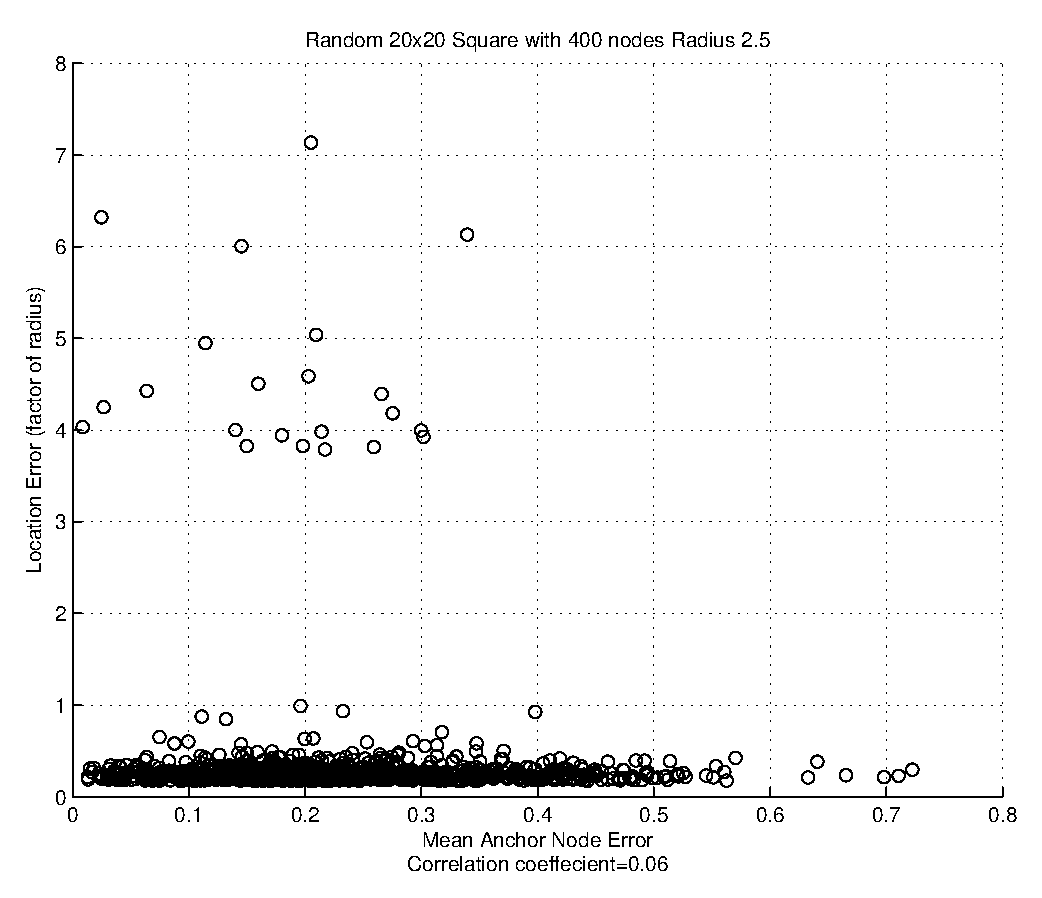
\includegraphics[width=0.9\textwidth]{numneighbors/AnchorSetErrorVsError}
		\end{figure}
	\end{column}
\end{columns}
\end{block}
\end{frame}

\begin{frame}{The Worst Case}
\begin{block}{What does it look like}
\begin{columns}
	\begin{column}[T]{0.3\textwidth}
		\begin{itemize}
		\item Criss-cross effect
		\item Anchor nodes themselves are not affected
		\item Could keep points inside known region, but does not help that much
		\end{itemize}
		\vfill
	\end{column}
	\begin{column}[T]{0.7\textwidth}
		\begin{figure}
			\centering
				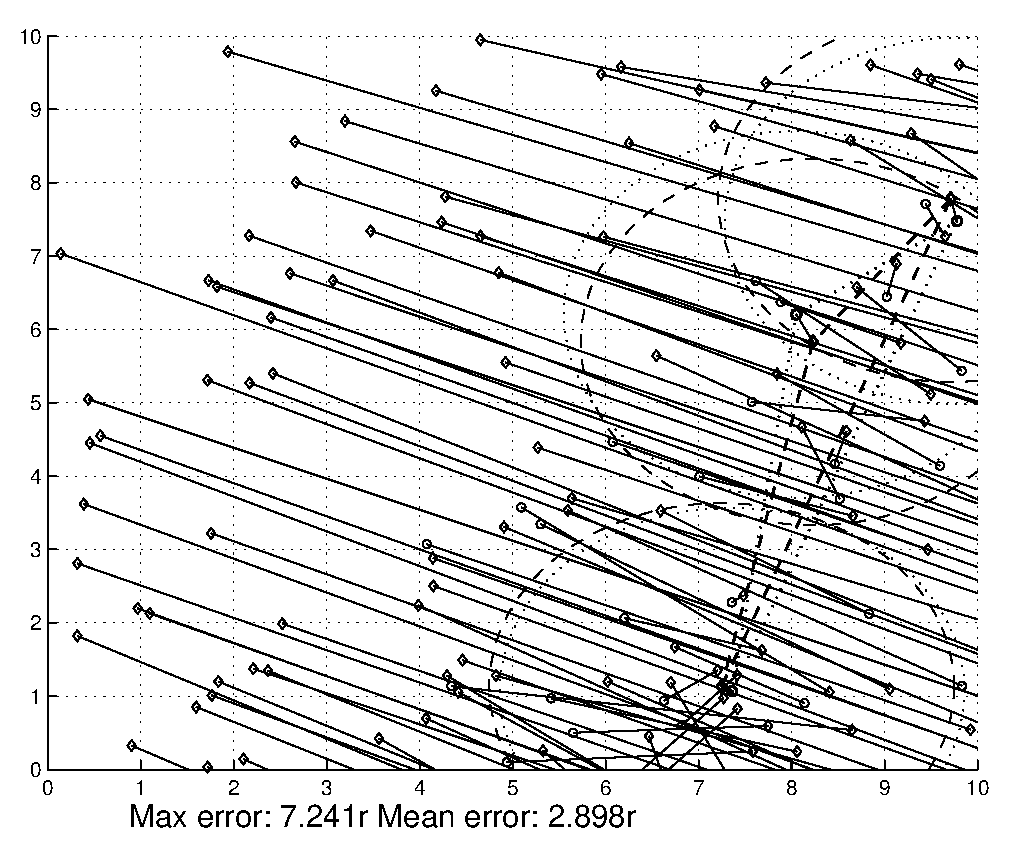
\includegraphics[width=0.7\textwidth]{AS6NetworkDiff9}
		\end{figure}
	\end{column}
\end{columns}
\end{block}
\end{frame}

\begin{frame}{The Worst Case}
\begin{block}{Avoiding it}
\begin{columns}
	\begin{column}[T]{0.3\textwidth}
		\begin{figure}
		  \centering
			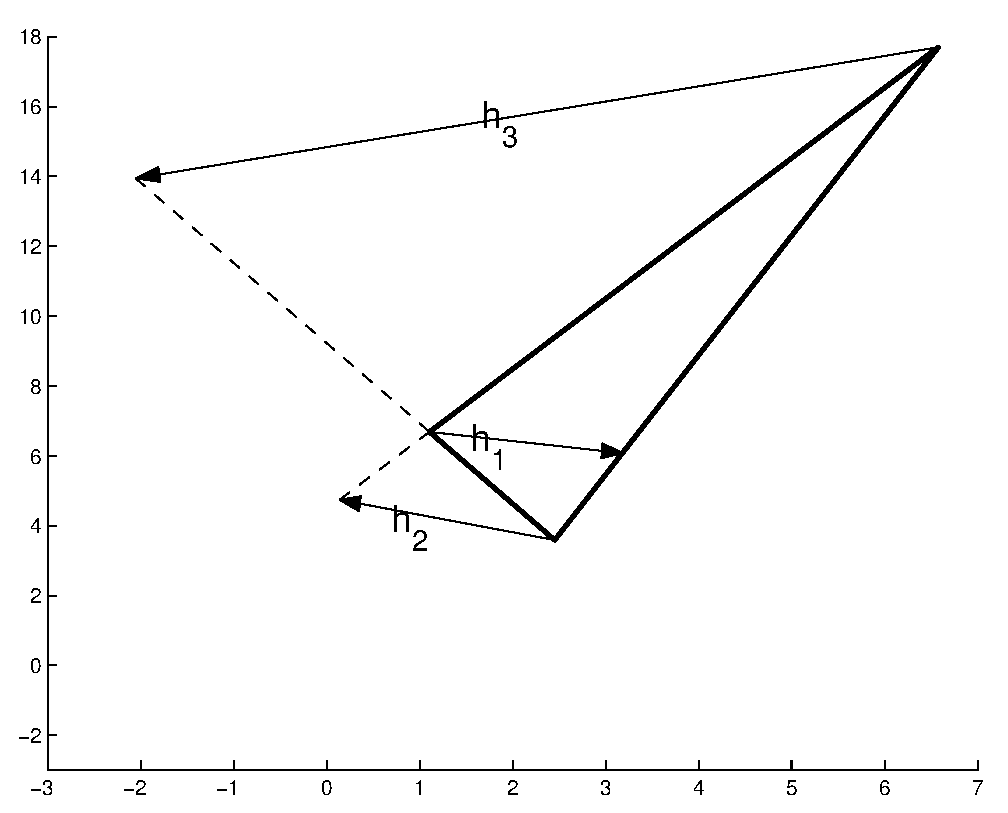
\includegraphics[width=0.8\textwidth]{SampleHeights}
		\end{figure}	
		\begin{itemize}
			\item Minimum anchor triangle heights
			\item[$\Rightarrow$] Height must be at least the radio range
		\end{itemize}
		\vfill
	\end{column}
	\begin{column}[T]{0.7\textwidth}
		\begin{figure}
			  \centering
				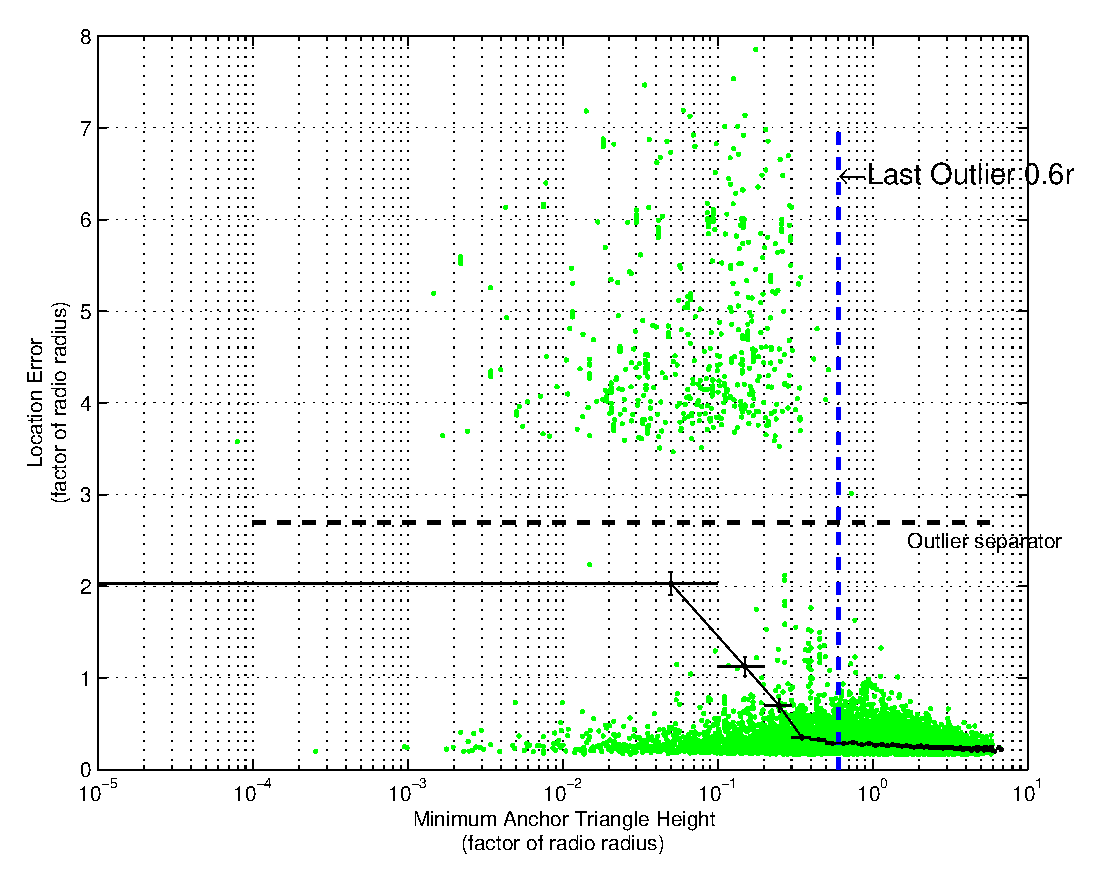
\includegraphics[width=0.95\textwidth]{HeightIndicator_square}
				\caption{95\% confidence intervals grouped in intervals of 0.1r}	
		\end{figure}
	\end{column}
\end{columns}
\end{block}
\end{frame}

\begin{frame}{The Normal Case}
\begin{block}{Making the best of it}
\begin{columns}
	\begin{column}[T]{0.3\textwidth}
		\begin{itemize}
			\item Sum of distance between anchor nodes
			\item The larger, the better
			\item[$\Rightarrow$] Sum must be at least 10 times the radio range
		\end{itemize}
		\vfill
	\end{column}
	\begin{column}[T]{0.7\textwidth}
		\begin{figure}
		  \centering
			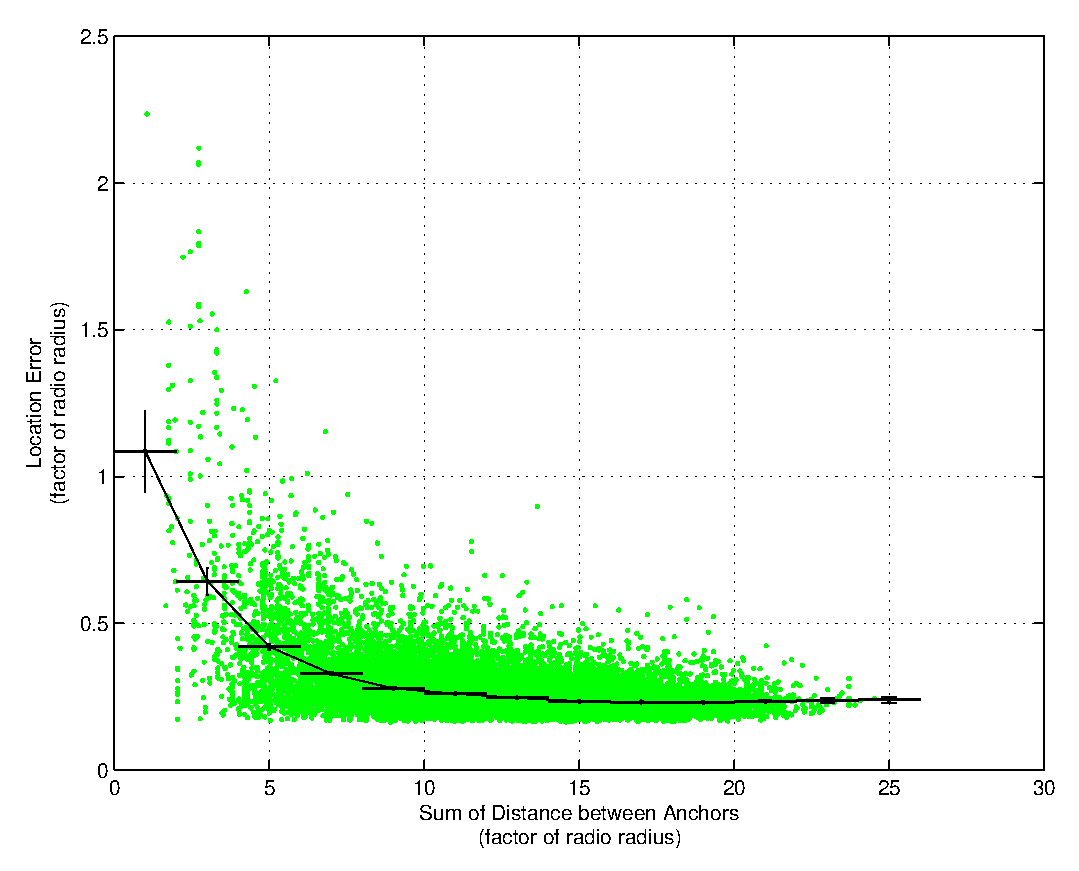
\includegraphics[width=0.7\textwidth]{SumOfDistanceIndicator_square}
			\caption{95\% confidence intervals of the mean in groups of 2 units, excluding outliers}
		\end{figure}
	\end{column}
\end{columns}
\end{block}
\end{frame}

\begin{frame}{Other Topologies}
\begin{block}{C-Shape}
		\begin{itemize}
			\item Similar results to square networks
			\item Minor increase in floor of error, as expected
		\end{itemize}
		\begin{figure}
			\centering
			\subfloat{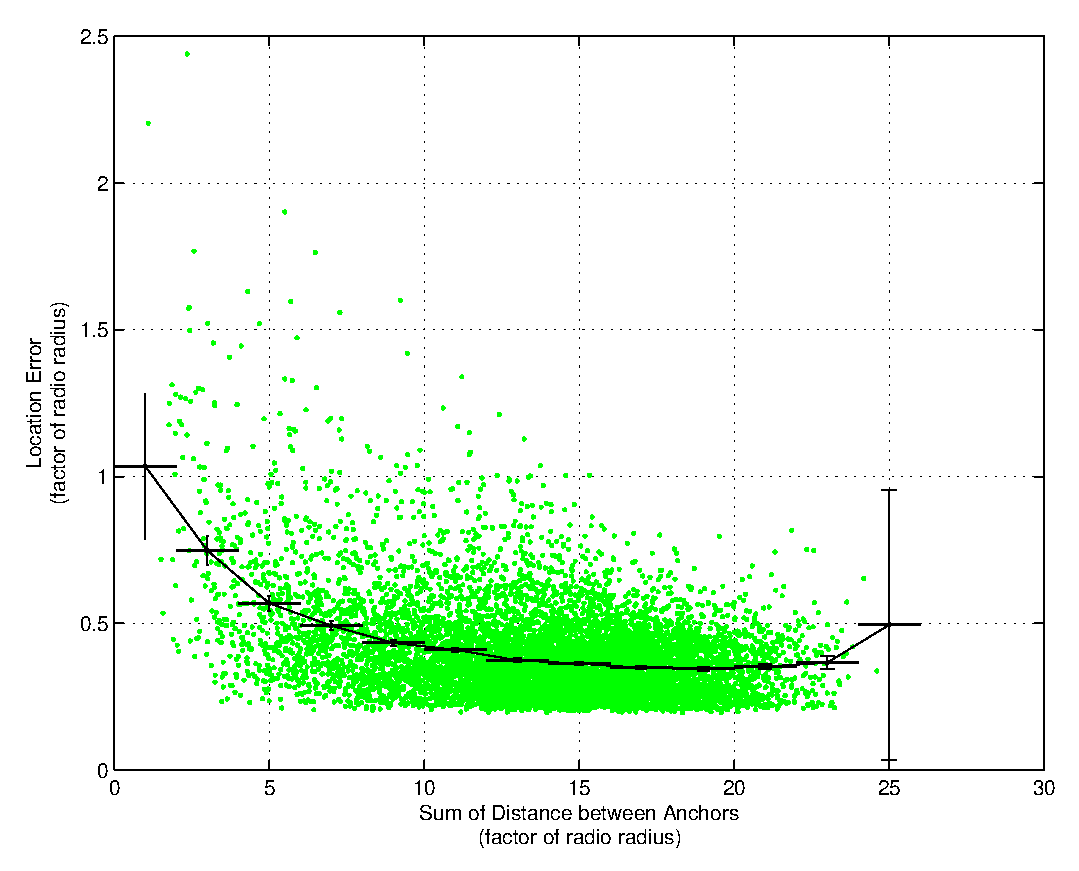
\includegraphics[width=0.5\textwidth]{cshape/SumOfDistanceIndicator_cshape}}~
			\subfloat{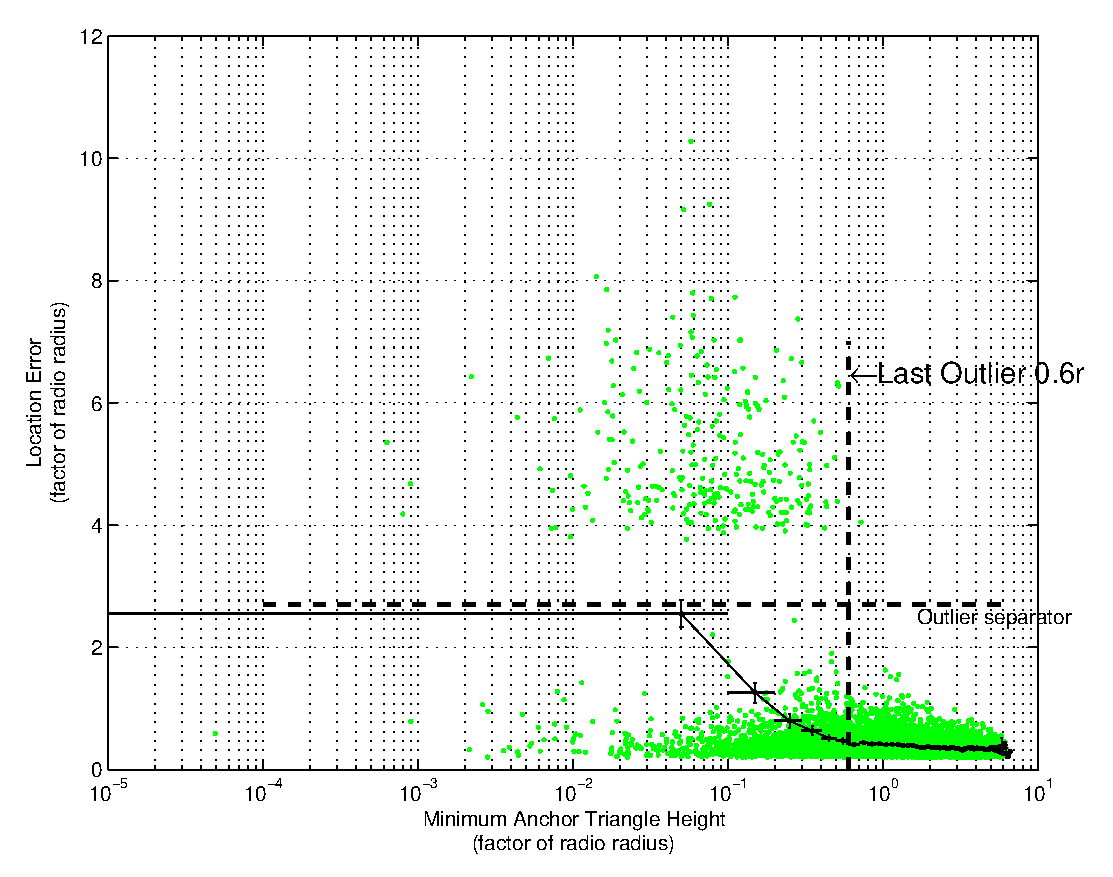
\includegraphics[width=0.5\textwidth]{cshape/HeightIndicator_cshape}}
		\end{figure}
\end{block}	
\end{frame}

\begin{frame}{Other Topologies}
\begin{block}{Pipeline}
\begin{columns}
	\begin{column}[T]{0.5\textwidth}
		\begin{figure}
			\centering
				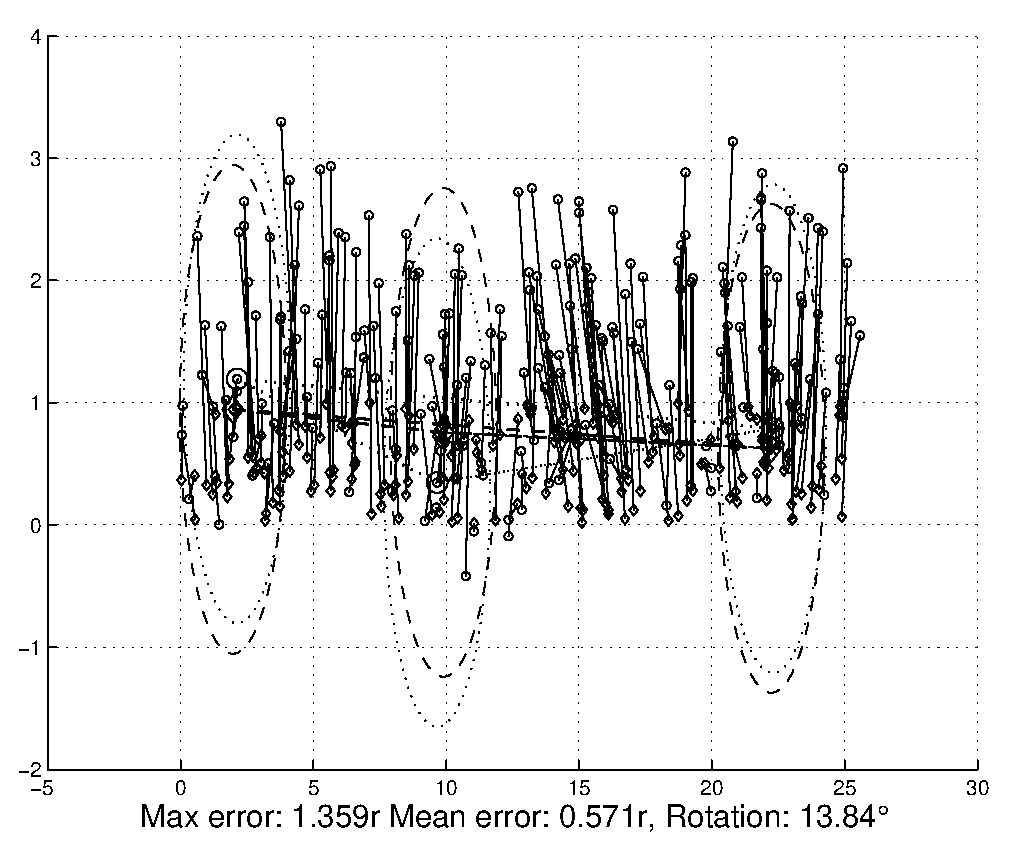
\includegraphics[width=\textwidth]{pipeline/spread}
		\end{figure}
	\end{column}
	\begin{column}[T]{0.5\textwidth}
		\begin{figure}
			\centering
				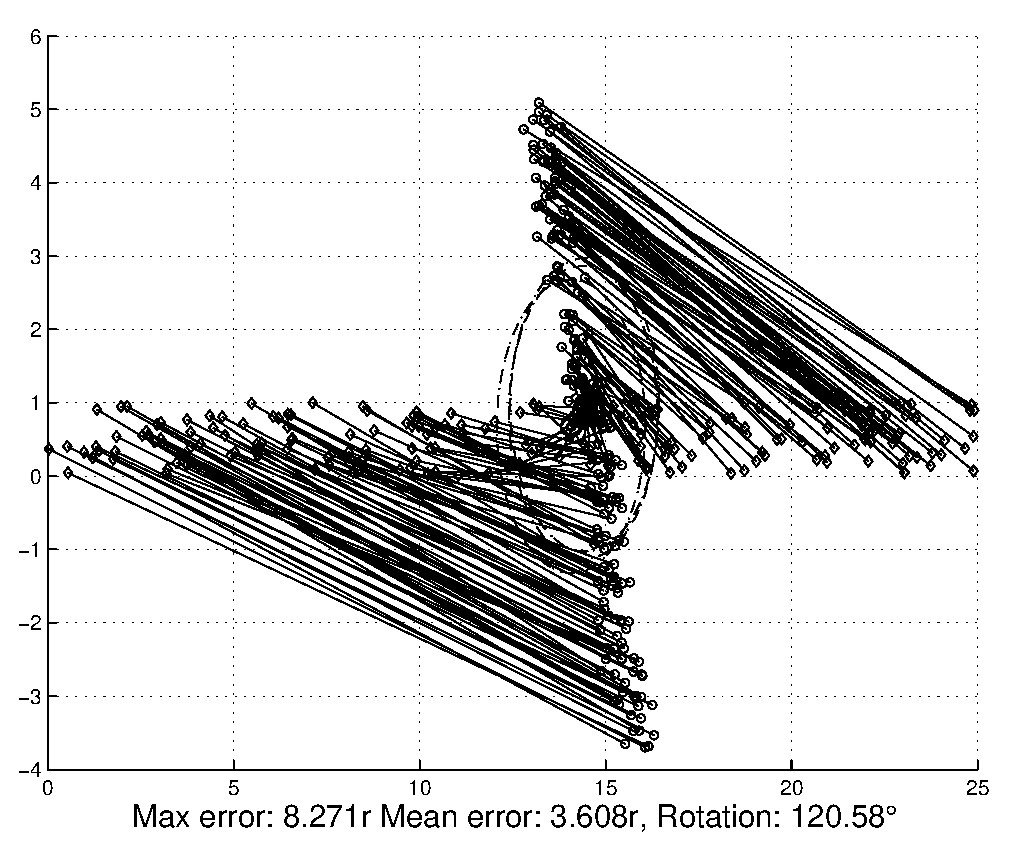
\includegraphics[width=\textwidth]{pipeline/clumped}
		\end{figure}
	\end{column}
\end{columns}
\end{block}
\end{frame}

\begin{frame}{Other Topologies}
\begin{block}{Pipeline}
\begin{columns}
	\begin{column}[T]{0.3\textwidth}
		\begin{itemize}
			\item Same as square networks, when deep enough
			\item Floor of error drops with depth
			\item Unlike previous, these plots show the outliers
			\item When shallow, outlier separation is non-existent
		\end{itemize}
		\vfill
	\end{column}
	\begin{column}[T]{0.7\textwidth}
		\begin{figure}
			\centering
				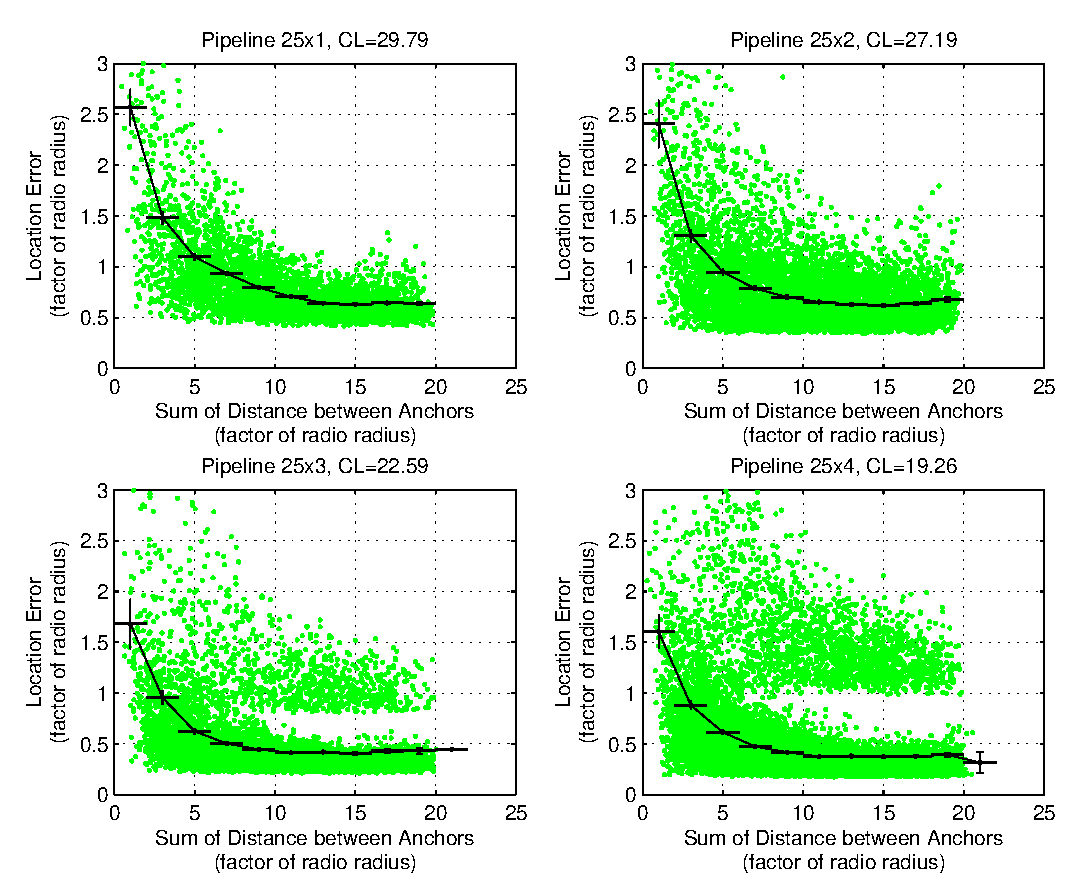
\includegraphics[width=0.9\textwidth]{pipeline/SumOfDistanceIndicator_pipes}
		\end{figure}
	\end{column}
\end{columns}
\end{block}	
\end{frame}

\begin{frame}{Other Topologies}
\begin{block}{Pipeline}
\begin{columns}
	\begin{column}[T]{0.3\textwidth}
		\begin{itemize}
			\item Impossible to meet minimum anchor triangle height criteria until depth of the pipeline grows
			\item Impossible to detect outliers
		\end{itemize}
		\vfill
	\end{column}
	\begin{column}[T]{0.7\textwidth}
		\begin{figure}
			\centering
				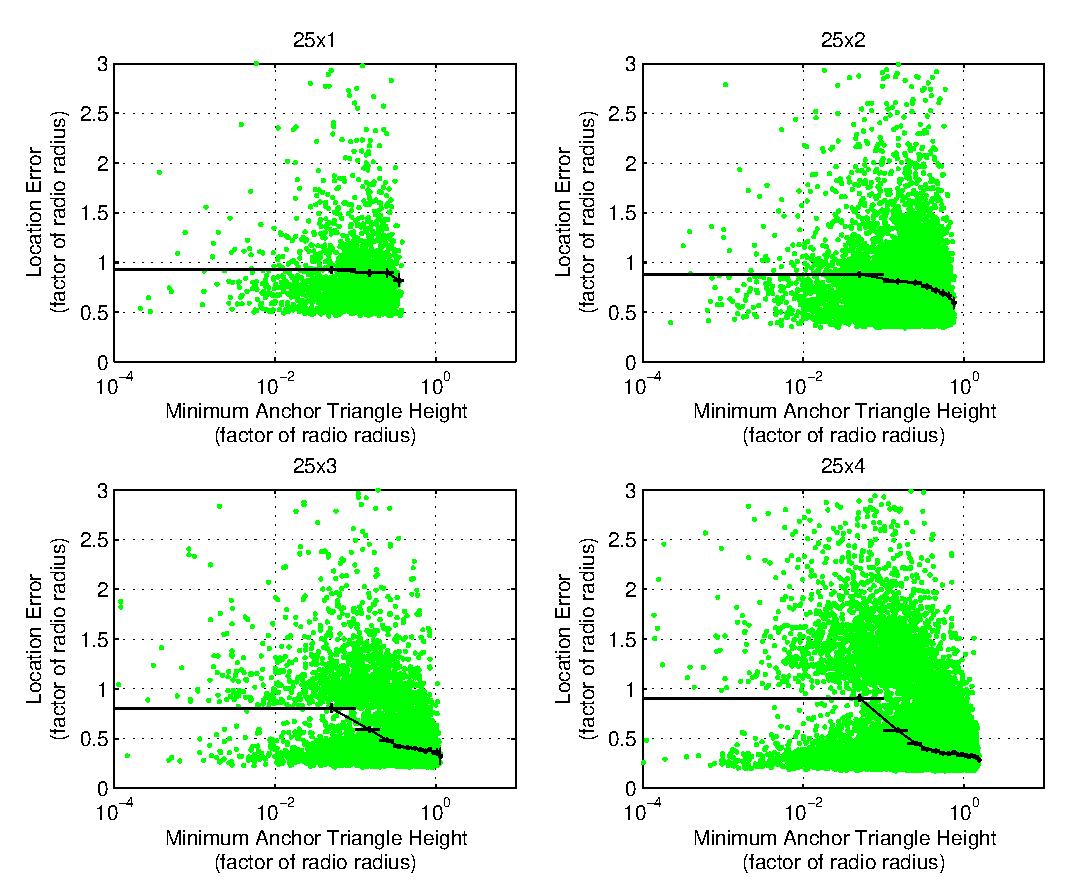
\includegraphics[width=0.9\textwidth]{pipeline/HeightIndicator_pipes}
		\end{figure}
	\end{column}
\end{columns}
\end{block}	
\end{frame}

\begin{frame}{Conclusions}
\begin{block}{Summary}
	\begin{itemize}
		\item[$\Rightarrow$] Sum of the distance between anchor nodes is at least ten times the radio range
		\item[$\Rightarrow$] Minimum height of the triangle formed by the anchor nodes is at least equal to the radio range
		\item[$\Rightarrow$] Not applicable to shallow pipeline topology
	\end{itemize}
\end{block}
\begin{block}{What's Next}
	\begin{itemize}
		\item Examination of the other factors
			\begin{itemize}
				\item Network connectivity
				\item CCA-MAP deployment options
			\end{itemize}
		\item Further examination of other topologies
		\item 3 dimensions (and more)
	\end{itemize}
\end{block}	
\end{frame}

\begin{frame}
\centerline{The End}
\end{frame}
% End of slides
\end{document}